%%=============================================================================
%% Analyse marketing Kriket
%%=============================================================================

\chapter{Growth hack toegepast op Kriket}
\label{ch:implementatie}

Het voorbeeld dat in het vorige hoofdstuk aangehaald wordt zal hier worden uitgewerkt. Zo kan men bewijzen dat het toepassen van growth hacking kan op niet-technologische bedrijven mogelijk is. 

Het referral systeem, genaamd Referral Candy, zal in de website van Kriket (\href{https://kriket.be}{kriket.be}) worden geïmplementeerd. Dit gebeurt in samenhang van het lanceren van een nieuw product, de \emph{discover box}.

\section{Stappenplan}
\label{sec:implementatie-stappenplan}

Het stappenplan voor deze specifieke implementatie is als volgt:

\begin{enumerate}
	\item Huidige situatie bekijken
	\item Google Analytics opzetten
	\item Referral Candy toevoegen aan de Shopify website
	\item Aanpassingen aan de webshop
	\item Growth hack online zetten
	\item Monitoring gedurende één maand
	\item Data analyseren: A/B test, verkoopcijfers, aantal bezoekers, enz.
	\item Conclusie: growth hack succesvol?
\end{enumerate}

Deze worden stap voor stap uitgeschreven op de volgende pagina's. 

\subsection{Huidige situatie bekijken} \label{sec:huidige-situatie-analyseren}

Hieronder staat een overzicht van de gebruikte technologieën en platformen.

\textbf{Webshop}
\begin{itemize}
	\item Shopify
\end{itemize}

\textbf{Data en analytics}
\begin{itemize}
	\item Shopify Analytics
\end{itemize}

\textbf{Sociale media platformen}
\begin{itemize}
	\item Facebook
	\item Instagram
\end{itemize}

Dit is een goede basis waaraan Google Analytics binnen \emph{Data en analytics} wordt toegevoegd en aan de webshop wordt de module voor het referral systeem toegevoegd.

\subsection{Google Analytics opzetten} \label{sec:google-analytics-opzetten}
Het koppelen van de Shopify website met Google Analytics is een eenvoudig proces. De Google account van Kriket werd gebruikt om een Analytics profiel aan te maken. De basis-koppeling stond klaar, maar Analytics werd nog niet ten volle gebruikt. Er waren geen doelen ingesteld en zo kan men moeilijk opvolgen wat de gebruikers op de website doen. Zodra de doelen zijn ingesteld kan men specifieke acties volgen en bekijken wanneer de gebruiker stopt in het proces van betaling.

De volgende doelen werden aangemaakt:
\begin{itemize}
	\item Added address
	\item Added payment info
	\item Added product to cart
	\item Added shipping info
	\item Checkout page
	\item Order completed
\end{itemize}

\subsection{Referral Candy toevoegen} \label{sec:referral-candy-toevoegen}
De Shopify applicatie Referral Candy wordt toegevoegd en geconfigureerd naar de noden van Kriket. Het volgende concept wordt toegepast:

\emph{Arno} is heel tevreden van Kriket en wil het product aanraden aan zijn vriendin \emph{Bonnie}. Bonnie krijgt volgende URL van Arno opgestuurd via Facebook Messenger ``https://kriket.refr.cc/arno``. Bonnie is geïnteresseerd in het concept van Kriket en koopt via de link van Arno een discover box. Door de link van Arno te gebruiken heeft Bonnie 20\% kunnen besparen. Arno krijgt op zijn beurt ook voordeel en ontvangt 20\% korting op zijn volgende aankoop via een kortingscode die hij per mail krijgt opgestuurd.

Concreet gaat het als volgt in werking. De klant maakt kennis met het referral programma via:
\begin{itemize}
	\item Social media post met landingspagina (\href{https://kriket.referralcandy.com}{https://kriket.referralcandy.com})
	\item Pop-up na betaling
	\item E-mail die na aankoop wordt verstuurd
\end{itemize}

Via de pop-up en e-mail krijgt met de link meteen en deze kan dan gedeeld worden. Via de landingspagina moet men natuurlijk eerst een e-mailadres doorgeven zodat de kortingscode hier naar opgestuurd kan worden. 

\begin{figure}[h!]
	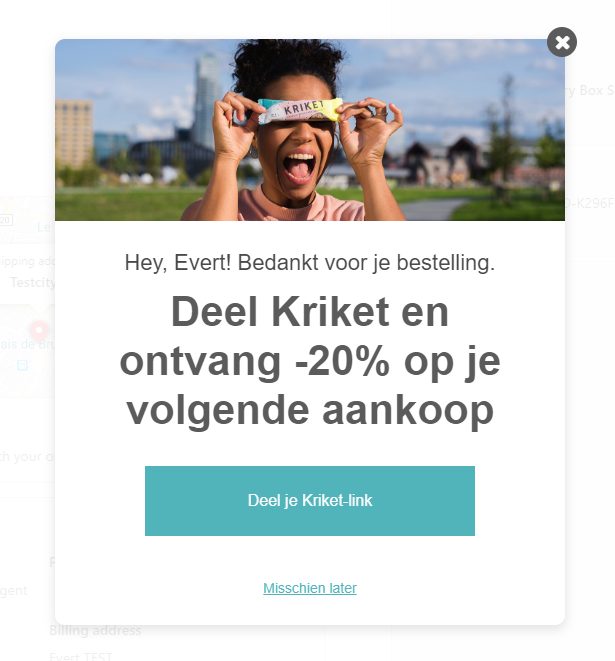
\includegraphics[width=80mm,scale=0.7]{img/referral-pop-up-1.png}
	\centering
	\caption{De pop-up na aankoop in de Kriket webshop.}
	\label{fig:referral-popup-webshop-1}
\end{figure}
\begin{figure}[h!]
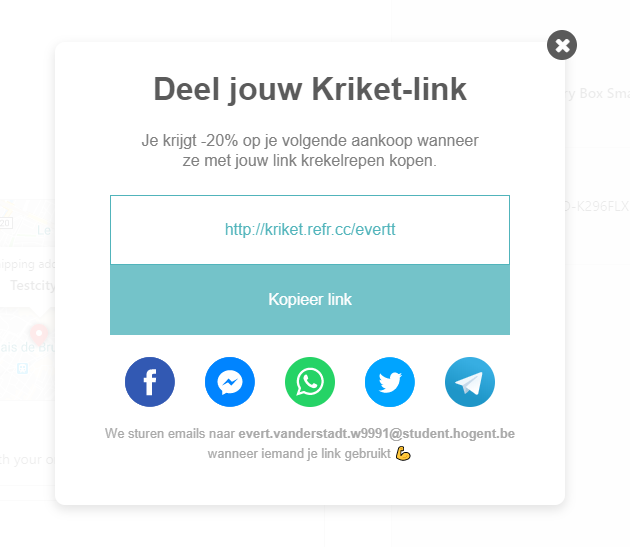
\includegraphics[width=80mm,scale=0.7]{img/referral-pop-up-2.png}
\centering
\caption{De link kan rechtstreeks uit de pop-up gekopieerd worden.}
\label{fig:referral-popup-webshop-2}
\end{figure}

Indien de link werd aangemaakt en gedurende 2 weken niet gebruikt werd, krijgt de klant een vriendelijke reminder e-mail met de boodschap om 20\% korting niet te laten vliegen.

Zodra de link (bijvoorbeeld: https://kriket.refr.cc/arno) wordt bezocht, gaat deze je doorsturen naar een pagina met als link bijvoorbeeld ``https://go.referralcandy.com/share/K296FLX`` (zie figuur \ref{fig:referral-share-page}). Op deze pagina ziet met de coupon code, die 20\% korting geeft op alle \emph{Discover Boxes}. Men kan de kortingscode kopiëren door op de tekst te klikken, maar deze wordt ook automatisch toegepast door op de CTA (Call To Action) - ``Bekijk de webshop`` te drukken. Via een aangepaste URL wordt de kortingscode bij het betaalproces automatisch ingevuld. Wanneer deze code gebruikt wordt zal de eigenaar van deze link (in dit voorbeeld - Arno), een link toegestuurd krijgen met een kortingscode voor hemzelf. Met deze code krijgt hij 20\% korting op alle items in de webshop.

\begin{figure}[h!]
	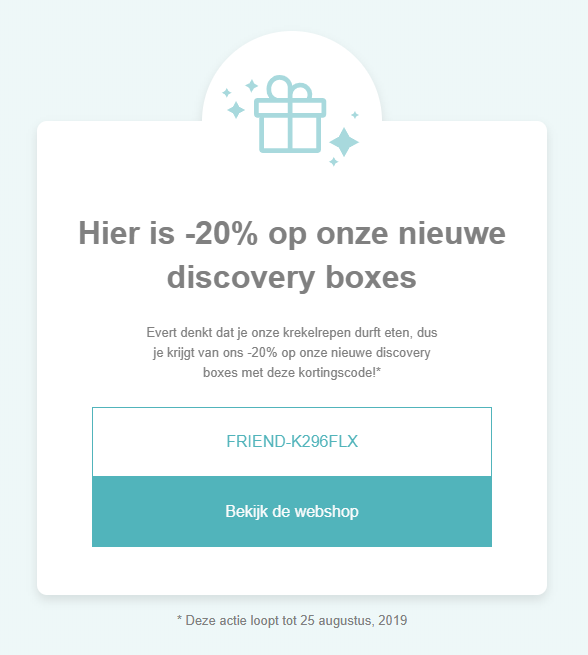
\includegraphics[width=80mm,scale=0.7]{img/referral-share-page.png}
	\centering
	\caption{Deze pagina krijgt de vriend(in) of kennis te zien wanneer de link (bijvoorbeeld \emph{https://kriket.refr.cc/arno}) wordt bezocht.}
	\label{fig:referral-share-page}
\end{figure}

Indien de gebruiker al zijn kortingscodes wil bekijken, kan deze dat doen via de link waar hij/zij de link heeft gecreëerd en gekopieerd. Bijvoorbeeld - \emph{https://kriket.referralcandy.com/MWGS976}, wanneer men daar op ``Jouw kortingscodes`` drukt gaat men naar een log-in pagina waar men vervolgens een wachtwoord kan creëren. Hierna kan men de pagina met kortingscodes bekijken - \emph{https://kriket.referralcandy.com/MWGS976/rewards} (zie figuur \ref{fig:referral-account.png}). Men kan hier ook zijn of haar persoonlijke link aanpassen (bijvoorbeeld \emph{https://kriket.refr.cc/evertv})

\begin{figure}[h!]
	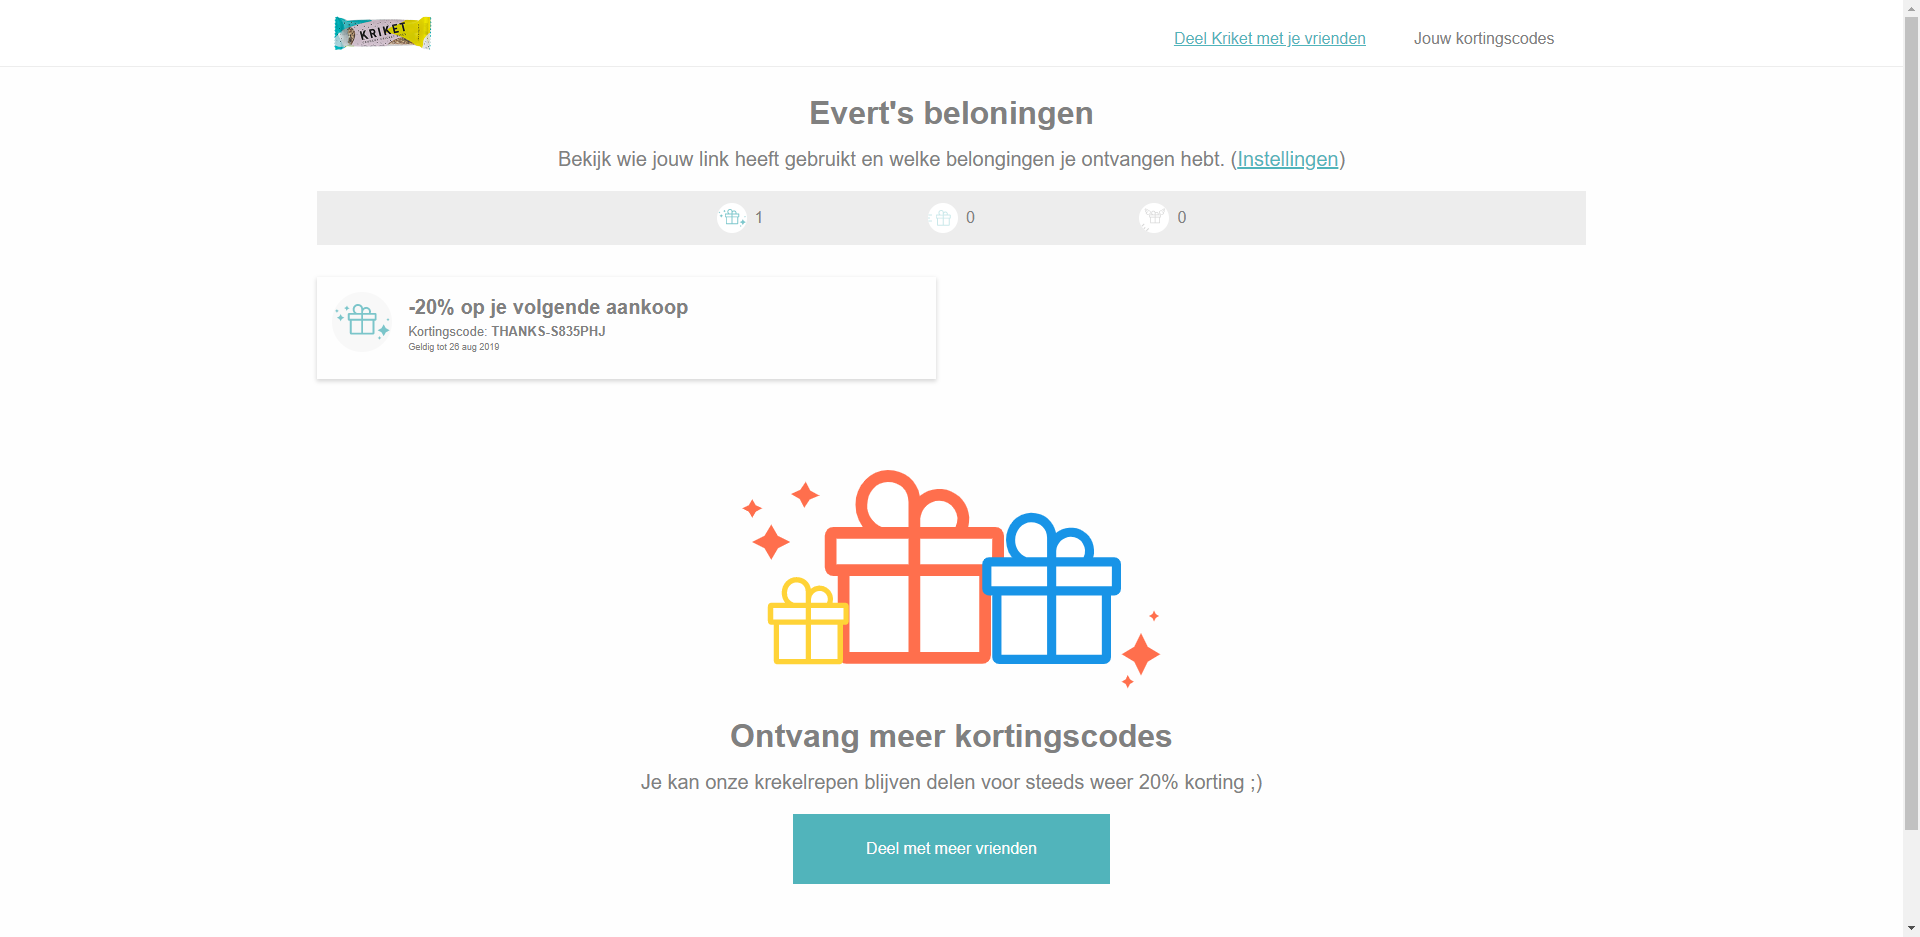
\includegraphics[width=\linewidth]{img/referral-account.png}
	\caption{Het overzicht van de kortingscodes van een gebruiker.}
	\label{fig:referral-account.png}
\end{figure}

Vanuit Referral Candy is er ook een nieuwe koppeling met Analytics toegevoegd. Een nieuwe \emph{property} genaamd ``Referral Program``, een \emph{property} is een onderdeel van een Analytics account. Een property kan een website, mobiele applicatie of dergelijke zijn. In dit geval is Referral Candy onze nieuwe applicatie die we koppelen aan de account. Deze staat dus los van de andere property, ``www.kriket.be``, die de eerder vermelde doelen bevat. Ze ontvangen de data van andere bronnen, de ene van Shopify en de andere van Referral Candy.

Tot slot was een groot deel van het opzetten goede tekst bedenken, copywriting is een vak apart - het marketing gedeelte is daar niet weg te denken. De teksten voor de pop-up, e-mails, landingspagina, overzicht pagina, ... enzovoort waren een belangrijk en tijdrovend onderdeel van het opzetten van Referral Candy. 

\subsection{Aanpassingen aan de webshop} \label{sec:aanpassingen-webshop}
Er worden 2 producten toegevoegd aan de webshop. ``DISCOVERY BOX LARGE`` en ``DISCOVERY BOX SMALL``, deze worden gebruikt bij het referral-programma.

\begin{figure}[h!]
	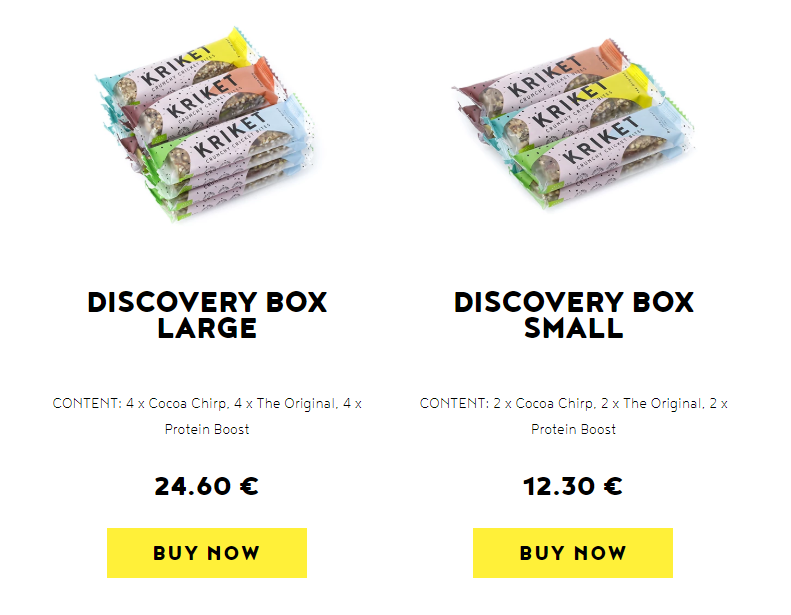
\includegraphics[width=\linewidth]{img/discovery-box-webshop.png}
	\caption{De twee nieuwe producten in de webshop.}
	\label{fig:discovery-box-webshop}
\end{figure}

Naast deze nieuwe producten toe te voegen worden de afbeeldingen verkleind. Het kleiner maken van de afbeeldingen zorgt voor een snellere laadtijd en een fijnere surf-ervaring op de webshop. Bij sommige producten is het verschil in bestand-grootte enorm - van 800Kb naar 100Kb. Tot wel 8 keer kleiner, het is een verschil dat zeker op valt.

\subsection{Growth hack online zetten} \label{sec:growth-hack-online-zetten}
Zodra het opzetten van alle voorgaande tools getest is kan de growth hack online gezet worden. Hierbij worden de twee sociale media platformen gebruikt. Langs Instagram en Facebook komen de fans en klanten van Kriket te weten dat het referral systeem beschikbaar is. 

Initieel wordt via Facebook een post gezet die aankondigt dat de actie van start gaat. Op het einde van de maand wordt er geëxperimenteerd met gesponsorde berichten op Instagram en Facebook. Via deze gerichte advertenties wordt de kans op nieuwe klanten vergroot.

Naast deze sociale media platformen wordt de klant ook op de hoogte gebracht via een pop-up na betaling en via e-mail. Deze ontvangt de klant na het plaatsen van een bestelling, zoals eerder vermeld (zie \ref{sec:referral-candy-toevoegen}). 

\subsection{Monitoring gedurende één maand} \label{sec:monitoring-gedurende-twee-weken}
Nu dat de growth hack online staat kan Google Analytics en de back-end tool van Referral Candy gebruikt worden voor de monitoring van deze growth hack. 

De growth hack werd gelanceerd op vrijdag 26 juli. Vanaf dat moment kregen de klanten een pop-up en e-mail na betaling in verband met het referral programma. 

De Facebook-post werd geplaatst op woensdag 7 augustus en de gesponsorde berichten kwamen hier kort achter.

\subsection{Data analyseren} \label{sec:data-analyseren}
De data uit het dashboard van Referral Candy, Google en Shopify Analytics zegt ons het volgende:

Van 26 juli tot 20 augustus werd volgende (interessante) data gecapteerd:

\textbf{Google Analytics}
\begin{itemize}
	\item Paginaweergaven: 2644	
	\item Sessies: 852
	\item Gem. sessieduur: 1 min 40 sec
	\item Bezoekers: 660 (zie figuur \ref{fig:acquisitie-kanalen})
		\subitem Desktop: 370
		\subitem Mobile: 270
		\subitem Tablet: 20
	\item Taal:
		\subitem NL: 45,17\%
		\subitem EN: 30,36\%
		\subitem DE: 7,25\%
		\subitem FR: 7,25\%
		\subitem ES: 1,81\%
\end{itemize}
\textbf{Shopify}
\begin{itemize}
	\item Sessies: 102 (93 bezoekers)
		\subitem Desktop: 59
		\subitem Mobile: 39
		\subitem Tablet: 4
	\item Orders voltooid: 23
	\item Totale verkoop: EUR 673,10
	\item Conversie ratio  (zie figuur \ref{fig:conversie-ratio-trechter})
		\subitem Product toegevoegd aan winkelmandje: 36,27\% (35 sessies)
		\subitem Betaling bereikt: 30,39\% (31 sessies)
		\subitem Conversies: 19,61\% (20 sessies)
	\item Populairste item: Discovery Box Large
\end{itemize}
\textbf{Referral Candy}
\begin{itemize}
	\item E-mails verstuurd: 48 (35 invite, 13 reminder)
	\item Link clicks: 25
	\item Social media shares: 13 (met 25 clicks)
	\item Webshop bezoeken: 16
	\item Aankopen via referral: 5
	\item Referral omzet: EUR 90,00 (zie figuur \ref{fig:directe-referral-verkoop})
\end{itemize}

\begin{figure}
	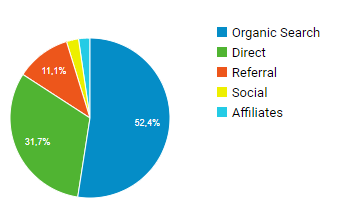
\includegraphics[]{img/acquisitie-kanalen.png}
	\centering
	\caption{De top acquisitie kanalen tussen 26 juli en 20 augustus.}
	\label{fig:acquisitie-kanalen}
\end{figure}


\begin{figure}
	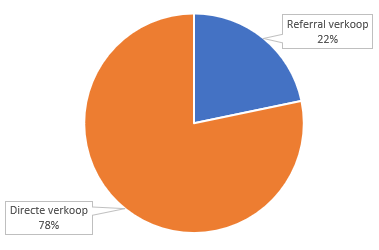
\includegraphics[scale=0.9]{img/directe-referral-verkoop.png}
	\centering
	\caption{Directe (18 orders) en referral (5 orders) verkoop in een cirkeldiagram.}
	\label{fig:directe-referral-verkoop}
\end{figure}

\begin{figure}
	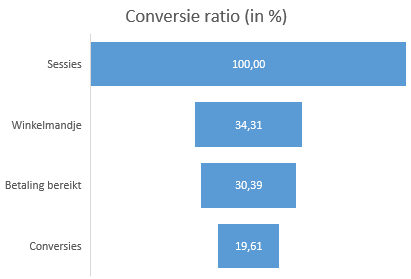
\includegraphics[scale=0.9]{img/conversie-ratio-trechter.png}
	\centering
	\caption{Conversie ratio is 19,61\%, dat wil zeggen dat bijna 1 op 5 sessies eindigt in een aankoop.}
	\label{fig:conversie-ratio-trechter}
\end{figure}

De verkoop data werd enkel uit Shopify gehaald en niet uit Google Analytics. Dit werd gedaan omdat Shopify de data direct bij de bron verkrijgt, Google Analytics kan minder accuraat zijn doordat het in deze situatie werkt met pagina bezoeken. Zo zal Google Analytics kijken naar \emph{/checkout/thank\_you} om te besluiten of er een betaling is gebeurd en Shopify krijgt deze data met 100\% zekerheid binnen omdat deze de betalingen opvolgt. In de tijdsspanne van 26 juli tot 20 augustus heeft Google Analytics 18 voltooide orders getracked en Shopify 23. Vandaar wordt voor deze data Shopify gebruikt.

Het grote verschil in aantal sessies bij Google Analytics en Shopify komt doordat Google Analytics alle sessies van bots mee rekent. Dit kan uitgezet worden bij de instellingen door ``Alle hits van bekende bots en spiders uitsluiten`` aan te vinken. Tijdens deze tests werd dit niet uitgezet en daardoor is er een groot verschil. We werken om deze reden vooral met de percentages en de exacte data uit Shopify.

\begin{figure}
	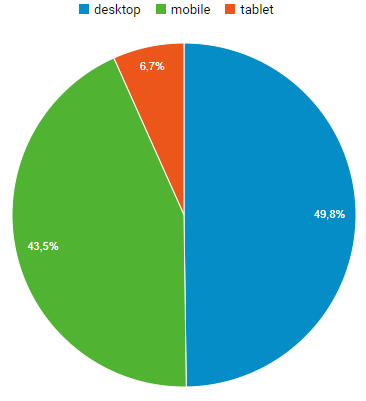
\includegraphics[scale=0.7]{img/sessies-per-apparaat.png}
	\centering
	\caption{Verdeling van aantal sessies op gebruikte apparaten, een opvallend aantal mobiele gebruikers}
	\label{fig:sessies-per-apparaat}
\end{figure}

Deze data kunnen we vergelijken met dezelfde periode, maar voordat de growth hack in actie werd gezet. Bijvoorbeeld van 1 tot 25 juli, de vergelijking doen we best met verkoopcijfers. Enkele belangrijke cijfers vind je in de tabel hieronder.


\begin{tabular}{ |p{4cm}||p{3cm}|p{3cm}|  }
	\hline
	\multicolumn{3}{|c|}{Vergelijking voor en tijdens growth hack} \\
	\hline
	Periode & 1 - 25 juli &26 juli - 20 aug\\
	\hline
	Sessies   & 66    &102\\
	Terugkerende bezoekers   & 42,86\%    &26,09\%\\
	Orders voltooid&   14  & 23\\
	Conversie ratio &21,21\% & 19,61\%\\
	Totale verkoop    &693,40 EUR & 673,10 EUR\\
	Gem. order waarde    &49,53  EUR& 30,81 EUR\\
	\hline
\end{tabular}

\subsection{Conclusie: growth hack succesvol?} \label{sec:conclusie-growth-hack-succesvol}
We kunnen uit de laatste tabel hierboven afleiden dat de growth hack vooral voor meer orders heeft gezorgd. Na verder onderzoek zien we een gemiddelde van 13 à 17 orders per maand voor de afgelopen maanden. De orders van het referral programma zijn dus bijkomende orders.

Verder is het aantal sessies enorm gestegen, dit mede door de advertenties via Facebook Ads. De klanten van Kriket zijn mogelijks na 1 maand nog niet genoeg vertrouwd met het referral programma, waardoor ze het nog niet willen gebruiken. Een langere periode zal er voor zorgen dat ze vertrouwd zijn met het systeem. Wanneer ze de nood aan nieuwe krekelrepen voelen, zullen ze denken aan de mogelijkheid om 20\% korting te verkrijgen via dit systeem.

Was de growth hack succesvol? Op het eerste zicht is er niet gigantisch veel veranderd tijdens deze maand, maar het aantal nieuwe bezoekers en nieuwe klanten zorgt waarschijnlijk voor stabiele groei de volgende maanden. 

